\documentclass[11pt,a4paper]{article}
\usepackage[margin=1.75cm,top=1.55cm,bottom=1.55cm]{geometry}
\usepackage[T1]{fontenc}
\usepackage[utf8]{inputenc}
\usepackage{helvet}
\renewcommand{\familydefault}{\sfdefault}
\usepackage{xcolor,graphicx,tabularx,array,enumitem,tikz,hyperref,fancyhdr,amssymb}
\usetikzlibrary{arrows.meta,positioning}
\definecolor{Fondo}{HTML}{F2EDE4}
\definecolor{Suave}{HTML}{E9E0D2}
\definecolor{Tinta}{HTML}{1A150F}
\definecolor{Sec}{HTML}{574C3D}
\definecolor{Acento}{HTML}{BD3A1E}
\definecolor{Verde}{HTML}{1E332C}
\hypersetup{colorlinks=true,urlcolor=Acento}
\pagestyle{fancy}\fancyhf{}
\fancyhead[L]{\small\bfseries TPO Store}
\fancyhead[R]{\small Primer checkpoint}
\fancyfoot[C]{\small Página \thepage\ de 4}
\renewcommand{\headrulewidth}{0.4pt}
\setlength{\parindent}{0pt}
\setlength{\parskip}{7pt}
\setlist[itemize]{leftmargin=6mm,itemsep=3pt,topsep=2pt}
\newcommand{\pagina}[2]{\vspace*{-3mm}{\color{Acento}\small\bfseries #1}\par{\color{Tinta}\LARGE\bfseries #2}\vspace{2mm}\hrule\vspace{5mm}}
\newcommand{\subt}[1]{\vspace{2mm}{\color{Verde}\large\bfseries #1}\par}
\newcommand{\caja}[1]{\begingroup\setlength{\fboxsep}{10pt}\colorbox{Fondo}{\parbox{\dimexpr\textwidth-20pt\relax}{#1}}\endgroup}
\newcommand{\bien}{\textcolor{Verde}{\checkmark}}
\newcolumntype{Y}{>{\raggedright\arraybackslash}X}
\begin{document}

\pagina{DESARROLLO DE APLICACIONES II}{TPO Store: qué hicimos hasta ahora}

\caja{\Large\bfseries En una frase\\[3pt]
\large Creamos una tienda online que muestra productos reales y obtiene la información desde un backend hecho con Jakarta EE.}

\subt{¿Qué puede hacer una persona?}
\begin{itemize}
  \item Ver el catálogo y las categorías.
  \item Buscar productos por nombre, marca o código.
  \item Filtrar por categoría, precio y disponibilidad.
  \item Ordenar los resultados.
  \item Abrir el detalle de un producto.
\end{itemize}

\begin{center}
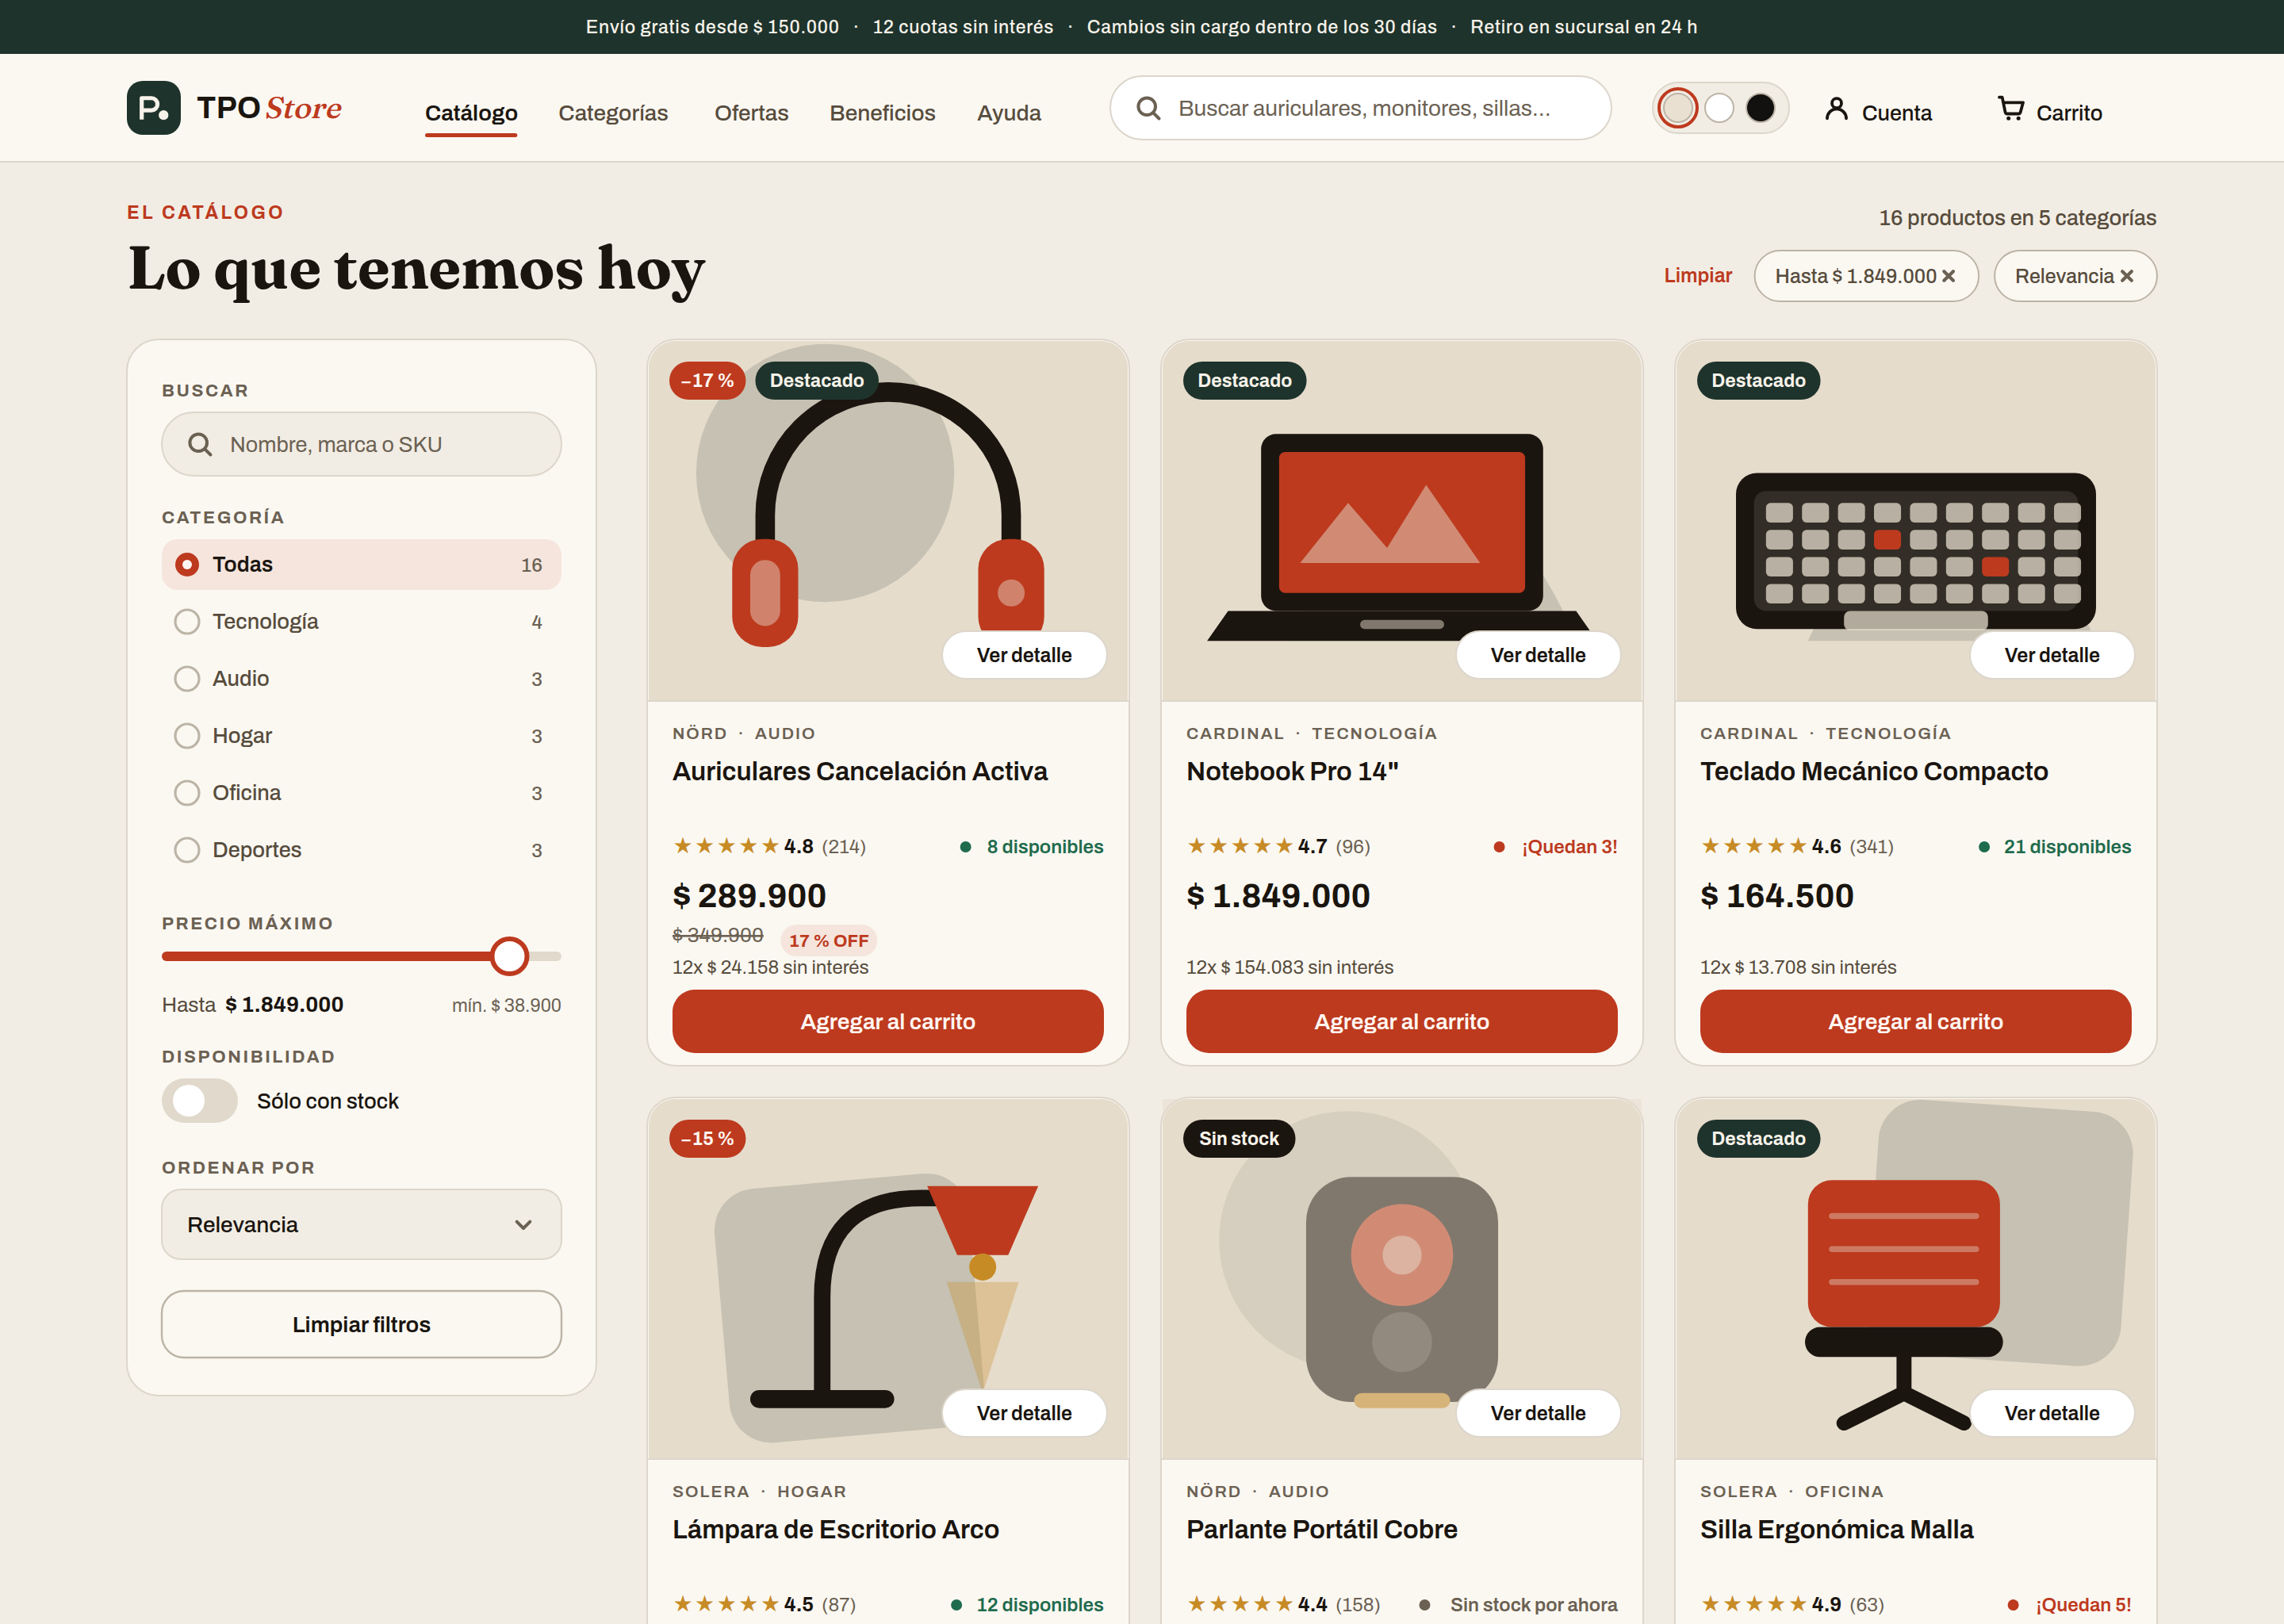
\includegraphics[width=.74\textwidth]{figma-checkpoint-1/exports/01-catalogo-desktop.png}
\end{center}

\subt{¿Qué presentamos en este checkpoint?}
No intentamos terminar todo el e-commerce. Para esta primera entrega mostramos
\textbf{una parte pequeña, pero completa y funcionando}: el Catálogo.

\begin{center}
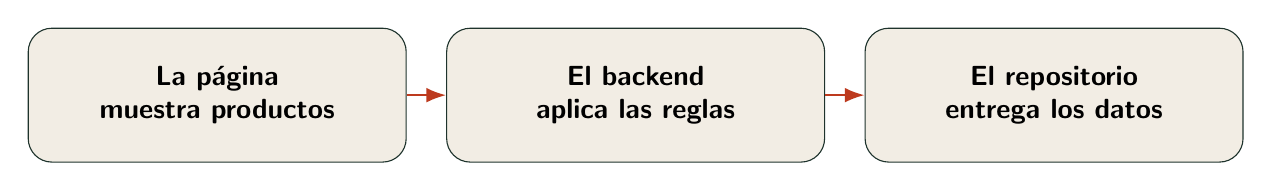
\begin{tikzpicture}[node distance=5mm,
 paso/.style={draw=Verde,rounded corners=3mm,fill=Fondo,minimum width=48mm,minimum height=17mm,align=center,font=\bfseries},
 flecha/.style={-{Latex[length=2.5mm]},thick,color=Acento}]
\node[paso] (a) {La página\\muestra productos};
\node[paso,right=of a] (b) {El backend\\aplica las reglas};
\node[paso,right=of b] (c) {El repositorio\\entrega los datos};
\draw[flecha] (a)--(b); \draw[flecha] (b)--(c);
\end{tikzpicture}
\end{center}

\vfill
\textbf{Equipo:} Rodrigo, Nicolás, Tomás, Iván y Fol.

\newpage
\pagina{ORGANIZACIÓN DEL SISTEMA}{Los componentes, explicados fácil}

Un componente es una parte del sistema que tiene un trabajo concreto. Es parecido
a dividir una empresa en sectores: ventas no debería encargarse también del depósito,
los pagos y la atención al cliente.

\caja{\textbf{Para la primera entrega:} identificamos ocho componentes, pero sólo
implementamos Catálogo. Los demás se van agregando de a poco en las próximas entregas.}

\renewcommand{\arraystretch}{1.45}
\begin{tabularx}{\textwidth}{>{\bfseries\color{Verde}}p{34mm}Y}
Usuarios & Registro, inicio de sesión y permisos.\\
Catálogo & Muestra productos, categorías, precios y búsquedas. \textbf{Ya funciona.}\\
Inventario & Controla cuánto stock hay y reserva unidades.\\
Carrito & Recuerda qué productos eligió cada cliente.\\
Pedidos / Checkout & Confirma la compra y coordina los pasos necesarios.\\
Pagos & Se comunica con la pasarela de pago.\\
Facturación & Genera el comprobante usando un sistema externo.\\
Notificaciones & Envía avisos cuando una compra cambia de estado.\\
\end{tabularx}

\subt{¿Por qué separar el sistema así?}
\begin{itemize}
  \item Cada parte tiene una responsabilidad clara.
  \item Podemos cambiar una parte sin romper todo el proyecto.
  \item El equipo puede trabajar de forma ordenada.
  \item Es más fácil probar y explicar el funcionamiento.
\end{itemize}

\subt{Qué se agregará después}
\begin{tabularx}{\textwidth}{>{\bfseries}p{40mm}Y}
Próxima entrega & Carrito, usuarios, seguridad y pedidos.\\
Entregas posteriores & Mensajería, pago REST, facturación SOAP y transacciones.\\
\end{tabularx}

\vfill
\caja{\textbf{Idea importante:} la consigna no pide implementar los ocho componentes
en el primer checkpoint. Pide identificarlos y demostrar al menos uno completo.}

\newpage
\pagina{PRIMER COMPONENTE}{Cómo funciona el Catálogo}

Cuando alguien busca un producto suceden tres pasos:

\begin{center}
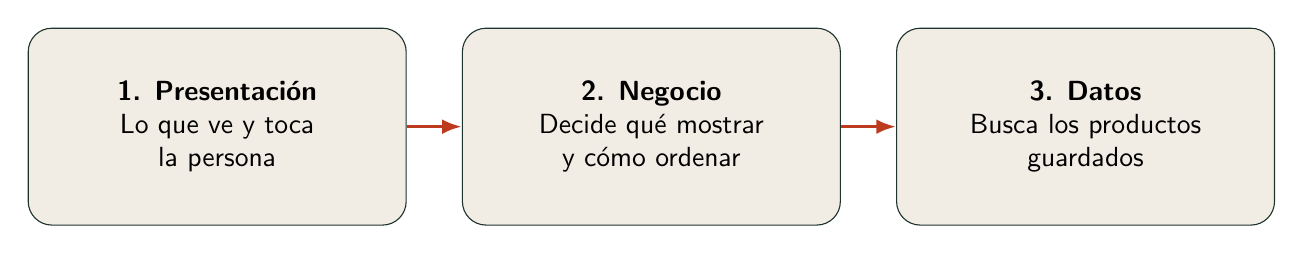
\begin{tikzpicture}[node distance=7mm,
 paso/.style={draw=Verde,rounded corners=3mm,fill=Fondo,minimum width=48mm,minimum height=25mm,align=center},
 flecha/.style={-{Latex[length=2.5mm]},very thick,color=Acento}]
\node[paso] (a) {\textbf{1. Presentación}\\Lo que ve y toca\\la persona};
\node[paso,right=of a] (b) {\textbf{2. Negocio}\\Decide qué mostrar\\y cómo ordenar};
\node[paso,right=of b] (c) {\textbf{3. Datos}\\Busca los productos\\guardados};
\draw[flecha] (a)--(b); \draw[flecha] (b)--(c);
\end{tikzpicture}
\end{center}

\subt{1. Presentación}
Es la tienda que vemos en el navegador: buscador, filtros, tarjetas y detalle.
También recibe y devuelve las respuestas de la API.

\subt{2. Negocio}
Acá viven las reglas. Por ejemplo: no mostrar productos inactivos, buscar sin
importar los acentos, filtrar por stock y ordenar por precio.

\subt{3. Datos}
Es la parte que entrega los productos. Hoy usa un archivo en memoria. Más adelante
se reemplazará por una base de datos con JPA sin cambiar las reglas del Catálogo.

\subt{¿Qué significa “stateless”?}
Es una palabra técnica que significa \textbf{“no necesita recordar a cada usuario”}.
Cada búsqueda llega completa y puede resolverse por sí sola.

Por ejemplo, para buscar notebooks no hace falta recordar lo que esa persona hizo
cinco minutos antes. En cambio, el futuro Carrito sí tendrá que recordar qué agregó
cada cliente, por eso será stateful.

\caja{\textbf{Cómo decirlo en la defensa:}\\
“Catálogo es stateless porque cada consulta contiene toda la información necesaria.
No guarda una conversación por usuario. WildFly puede reutilizar sus instancias.”}

\subt{Qué tecnología usamos}
\begin{tabularx}{\textwidth}{>{\bfseries}p{34mm}Y}
Java 17 & Lenguaje del backend.\\
Jakarta EE & Herramientas para crear los componentes y la API.\\
WildFly & Servidor donde corre realmente la aplicación.\\
Maven & Compila, prueba y arma el archivo \texttt{ecommerce.war}.\\
HTML, CSS y JS & Construyen la tienda que ve el usuario.\\
\end{tabularx}

\newpage
\pagina{DEMOSTRACIÓN}{Qué mostrar y dónde encontrarlo}

\subt{Guion corto para la demo}
\begin{enumerate}[leftmargin=7mm,itemsep=4pt]
  \item Abrir la tienda y mostrar los productos.
  \item Buscar “notebook”.
  \item Filtrar por categoría y por stock.
  \item Cambiar el orden de los resultados.
  \item Abrir el detalle de un producto.
  \item Explicar el recorrido: pantalla $\rightarrow$ reglas $\rightarrow$ datos.
\end{enumerate}

\subt{Cómo ejecutar el proyecto}
\caja{\ttfamily
cd TPO\\
export JAVA\_HOME=/usr/lib/jvm/java-17-openjdk-amd64\\
./mvnw clean test package
}

Después se copia \texttt{target/ecommerce.war} en WildFly y se abre:

\begin{center}
\url{http://localhost:8080/ecommerce/}
\end{center}

\subt{Resultados comprobados}
\begin{tabularx}{\textwidth}{p{9mm}Y}
\bien & Compilación correcta y archivo WAR generado.\\
\bien & 12 pruebas aprobadas, sin fallas.\\
\bien & Catálogo funcionando dentro de WildFly.\\
\bien & Búsqueda, filtros, categorías y detalle funcionando.\\
\bien & Los errores se muestran con un mensaje claro.\\
\bien & Diseño adaptable a computadora y celular.\\
\end{tabularx}

\subt{Enlaces}
\begin{tabularx}{\textwidth}{>{\bfseries}p{31mm}Y}
Repositorio & \url{https://github.com/nievarodrigo/desarrollo-app-ii-tpo}\\
Trello & \url{https://trello.com/b/gbrISl9W/desarrollo-de-aplicaciones-2-tpo}\\
Tienda pública & \url{https://landing-ecommerce-tau.vercel.app}\\
Prototipo & Carpeta \texttt{figma-checkpoint-1/}\\
\end{tabularx}

\subt{Uso de inteligencia artificial}
Se utilizó IA para ayudar con partes repetitivas del código, revisar la organización,
crear pruebas y mejorar la documentación. El equipo revisó el resultado y debe poder
explicar cada decisión.

\vfill
\colorbox{Verde}{\parbox{\dimexpr\textwidth-20pt\relax}{\color{white}\large\bfseries
Resultado: tenemos un primer componente real, ordenado en capas, probado y listo
para seguir creciendo.}}

\end{document}

